\section{Teoria dos Grafos}

\par A teoria dos grafos foi criada pelo matemático suiço \textit{Leonhard} Euler no século XVIII com o propósito de solucionar um antigo problema, conhecido como as 7 pontes de \textit{Königsberg} \cite{harju_graph_theory}.

\par \textit{Königsberg}, atualmente conhecida como \textit{Kaliningrad}, era uma antiga cidade medieval cortada pelo rio \textit{Pregel} dividindo-a em 4 partes interligadas por 7 pontes. Ela era localizada na antiga Prússia, hoje, território Russo. O problema mencionado anteriormente consistia basicamente em atravessar toda a cidade, visitando todas as partes e utilizar todas as pontes desde que não repetisse uma das quatro partes ou uma das 7 pontes. A figura 2 ilustra o problema mencionado.

\newpage
% Imagem do problema das 7 pontes da teoria dos grafos
\begin{figure}[h!]
	\centerline{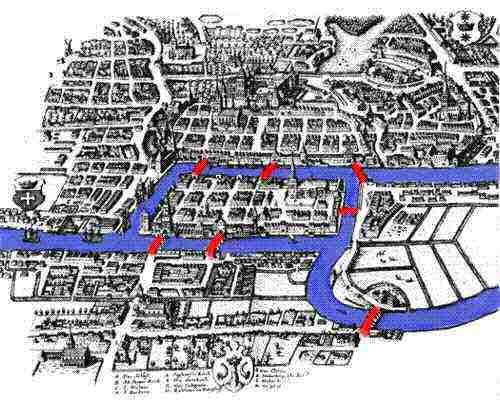
\includegraphics[height=0.26\textheight,width=0.8\textwidth]{./imagens/Konigsberg_7_bridges.jpg}}
	\caption[O problema das 7 pontes de \textit{Königsberg} ]
	{O problema das 7 pontes de \textit{Königsberg}. \textbf{Fonte:} \citeonline{paoletti_seven_bridges_konigsberg}}
	\label{fig:exemplo1}
\end{figure}

\par De acordo com \citeonline{bruggen_learning_neo4j}, para tentar solucionar o problema, Euler utilizou uma abordagem matemática ao contrário dos demais que tentaram utilizar a força bruta para solucionar tal problema, desenhando N números de diferentes possibilidades de rotas. Euler mudou o foco e passou a dar mais atenção ao número de pontes e não as partes da cidade. Através desta observação, foi possível perceber que realizar tal tarefa seria impossível, pois de acordo com sua teoria seria necessário possuir no mínimo mais uma ponte, uma vez que, o número de pontes era ímpar, não sendo possível realizar um caminho único e sem repetição. Desta forma, obteve-se a solução para este problema e criou-se o primeiro grafo no mundo.

\par \citeonline[p. 16]{rocha_algoritmos_particionamento_banco_dados_orientado_grafos} afirma que: 

\begin{citacao}
	um \textit{grafo G = (V,E)} consiste em um conjunto finito \textit{V} de vértices e um conjunto finito \textit{E} de arestas onde cada elemento \textit{E} possui um par de vértices que estão conectados entre si e pode ou não possuir um peso \textit{P}.
\end{citacao}

\par Esta é a definição formal de um grafo. A partir desta definição, é possível identificar, no problema mencionado anteriormente, os vértices que neste caso são as pontes e as arestas que por sua vez são as partes da cidade.

\par Segundo \citeonline{bondy_murty_graph_theory_with_applications}, muitas situações do mundo real podem ser descritas através de um conjunto de pontos conectados por linhas formando assim um grafo, como um centro de comunicações e seus links, ou as pessoas e seus amigos, ou uma troca de emails entre pessoas, entre outras. Isto é possível pois, de acordo com \citeonline{rocha_algoritmos_particionamento_banco_dados_orientado_grafos}, existem muitos problemas atualmente que podem ser mapeados para uma estrutura genérica possibilitando assim utilizar a teoria de grafos para tentar solucioná-los, tais como: rotas geográficas, redes sociais, entre outros.

%BANCA_QUALIFICACAO. Comentado este parágrafo, porém o mesmo retornará para a banca de qualificação
\par A figura 3 demostra de maneira visual um grafo, conforme ideia de \citeonline{bondy_murty_graph_theory_with_applications}, utilizando como exemplo o seguinte grafo \textit{G} = \{a, b, c, d, e, f, g, h\} e suas respectivas arestas \textit{E}$_g$ = \{(a, b), (a, h), (a, e), (b, f), (c, e), (c, d), (c, g), (d, e), (d, h), (d, g), (f, h)\}, sendo que os vértices serão representados por círculos e as arestas que os interligam por linhas.

%subscrito $_CARCTER_DESEJADO$

% Imagem do grafo simples - VOLTAR NA BANCA DE QUALIFICACAO
\begin{figure}[h!]
	\centerline{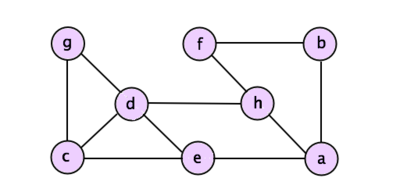
\includegraphics[scale=0.77]{./imagens/simple_graph.png}}
	\caption[Ilustração de uma representação gráfica de um simples grafo]
	{Ilustração de uma representação gráfica de um simples grafo. \textbf{Fonte:} \citeonline{rocha_algoritmos_particionamento_banco_dados_orientado_grafos}}
	\label{fig:exemplo1}
\end{figure}

%BANCA_QUALIFICACAO. Comentado este parágrafo, porém o mesmo retornará para a banca de qualificação
\par \citeonline{ruohonen_graph_theory} afirma que os grafos podem ser gerados com a possibilidade de permitir \textit{loops}\footnotemark[4] e arestas paralelas ou multiplas entre os vértices, obtendo um \textit{multigraph}. A figura 4 ilustra um simples \textit{multigraph}.

\footnotetext[4]{\textit{loops} - Uma aresta que interliga o mesmo vértice.}

% Imagem de um multigraph - VOLTAR NA BANCA DE QUALIFICACAO
\begin{figure}[h!]
	\centerline{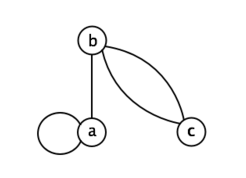
\includegraphics[scale=0.9]{./imagens/multigraph_example.png}}
	\caption[Ilustração de uma representação gráfica de um \textit{multigraph}]
	{Ilustração de uma representação gráfica de um \textit{multigraph}. \textbf{Fonte:} Adaptado de \citeonline{harju_graph_theory}}
	\label{fig:exemplo1}
\end{figure}

%BANCA_QUALIFICACAO. Comentado este parágrafo, porém o mesmo retornará para a banca de qualificação
\par Para \citeonline{harju_graph_theory}, os grafos podem ser direcionados (\textit{dígrafo}) ou não direcionados. Os  direcionados são aqueles cujos vértices ligados a uma aresta são ordenados e permitem que uma aresta que conecta os vértices \textit{x} e \textit{y} seja representada apenas de uma forma, sendo ela \{x, y\} ou \{y, x\}, ao contrário dos não direcionados que, para este mesmo caso, pode ser representado por ambas as formas \citeonline{rocha_algoritmos_particionamento_banco_dados_orientado_grafos}. A figura 5 demonstra um grafo direcionado.

% Imagem de um grafo direcionado - VOLTAR NA BANCA DE QUALIFICACAO
\begin{figure}[h!]
	\centerline{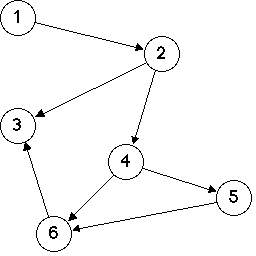
\includegraphics[scale=0.6]{./imagens/simple_digraph_graph.png}}
	\caption[Imagem de uma representação gráfica de um grafo direcionado]
	{Imagem de uma representação gráfica de um grafo direcionado. \textbf{Fonte:} \citeonline{robert_keller_acylic_graph}}
	\label{fig:exemplo1}
\end{figure}

\newpage %pular uma folha para que imagem fique na posição correta de acordo com a Joelma

Abaixo serão descritos alguns tipos de grafos existentes, de acordo com \citeonline{grafos_teoria_modelos_algoritimo_neto}.

\begin{itemize}
	\item \textbf{grafo simples:} são aqueles grafos que não possuem \textit{loops}, ou arestas paralelas;
	
	\item \textbf{grafo completo:} são aqueles cujo qualquer par de vértices são adjacentes;
	
	\item \textbf{caminho (travessia):} é uma sequência de vértices {v1, v2,...,vn} conectados por meio de arestas {e1 = {v1, v2}, {v1, v3}...,{vn, vm}};
	
	\item \textbf{grafo conexo:} são aqueles que, para qualquer par vértices {u,v}, há um caminho que os ligam;
	
\end{itemize} 
\par Este conteúdo teórico foi escolhido para ser utilizado neste trabalho pois,
este, visa equacionar o problema relacionado à busca por mão de obra, através do modelo utilizado pelas redes sociais. Isto é possível pois, como mencionado anteriormente por meio desta teoria é possível descrever várias situações do mundo real, e como ela é muito bem aplicada à redes sociais, inclusive grandes empresas desta área já a utilizam. Devido a estes motivos, esta teoria será  utilizada para auxiliar no desenvolvimento deste projeto.
